%%%% début de la page
\teteSndCorp


%%%% titre
\numeroActivite{1}
\titreTP{Dosage du sucre par étalonnage}

%%%% objectifs
\begin{objectifs}
  \item Connaître les règles de sécurités.
  \item Mesurer le taux de sucre dans un soda.
\end{objectifs}

%%%% contexte
\begin{encart}
  \emphase{Contexte :}
  
  Le sucre couramment présent dans notre alimentation est le saccharose.
  Cette espèce chimique peut entraîner des risques pour la santé si on en consomme trop.
  Il est donc important de pouvoir déterminer la quantité de sucre consommée par jour.
\end{encart}

\problematique{Comment déterminer la masse de saccharose présent dans un soda ?}


%%%% document
\begin{doc}{Dissolution du sucre dans l'eau}
  \vspace*{-0.6cm}
  \begin{enumerate}
      \item Peser une masse donnée de sucre avec une balance de précision.
      \item Mettre le sucre dans une fiole jaugée de 50 mL.
      \item Compléter la fiole jaugée jusqu'à mi-hauteur avec de l'eau distillée, agiter.
      \item Compléter jusqu'au trait de jauge avec de l'eau distillée.
      \item Verser le mélange dans un bêcher de 100 mL.
  \end{enumerate}
\end{doc}

\begin{doc}{Protocole de mesure d'une masse volumique}
  \vspace*{-0.6cm}
  \begin{enumerate}
    \item Peser un bêcher de 50 mL.
    \item Prélever 10 mL de l'espèce à mesurer avec une pipette jaugée, la verser dans le bêcher pesé.
    \item Peser le bêcher plein, en déduire la masse de l'espèce.
    \item En déduire la masse volumique.
  \end{enumerate}
\end{doc}


%%%% questions
\question{En utilisant le Document 1, préparer un mélange de 50 mL d'eau avec une masse $m =\!$\lignePointillee{0.05} g de sucre. \phantom{É}}{0}

\question{Pourquoi utilise-t-on une fiole jaugée comme verrerie ? 
%À l'aide du document 2, mesurer la masse volumique de 50 mL d'eau distillée avec une fiole jaugée et une éprouvette. Comparer.
}{1}

\question{En utilisant le document 2, mesurer la masse volumique du mélange préparé.}{0}

\question{Compléter la masse de sucre pesée et la masse volumique mesurée au tableau.}{0}

\question{Tracer la masse volumique en fonction de la masse de sucre dans 50 mL d'eau distillée.}{0}

\question{Le coca-cola a une masse volumique de \lignePointillee{0.05} g/L. \`A l'aide de la courbe tracée question 5, déduire la masse de sucre que ce soda contient.}{0}


%%%% conclusion
\begin{encart}
  \emphase{Conclusion :}
  Pendant ce TP, le mélange préparé était une \textbf{solution} avec une \textbf{concentration massique} de saccharose fixé.
  Cette concentration massique mesure la quantité de saccharose dissoute dans l'eau, à ne pas confondre avec la masse volumique de la solution d'eau sucrée.
  
  \bigskip
  La courbe tracée montrait la \textbf{relation de proportionnalité} entre masse volumique et concentration massique.
  Cette \textbf{courbe d'étalonnage} permet de déterminer la concentration massique de saccharose d'une solution inconnue en mesurant sa masse volumique.
\end{encart}

\includepdf[pages=26]{chapitre1_solution/papier_millimetre.pdf}

\feuilleBlanche
